% !TeX root = 00main.tex

%%%%%%%%%%%%%%%%%%%%%%%%%%%%%%%%%%%%%%%%%%%%%%%%%%%%
% Appendices
%%%%%%%%%%%%%%%%%%%%%%%%%%%%%%%%%%%%%%%%%%%%%%%%%%%
%
% Electronic schematics
%
\section{Electronic schematics}
\subsection*{Control box schematics}
%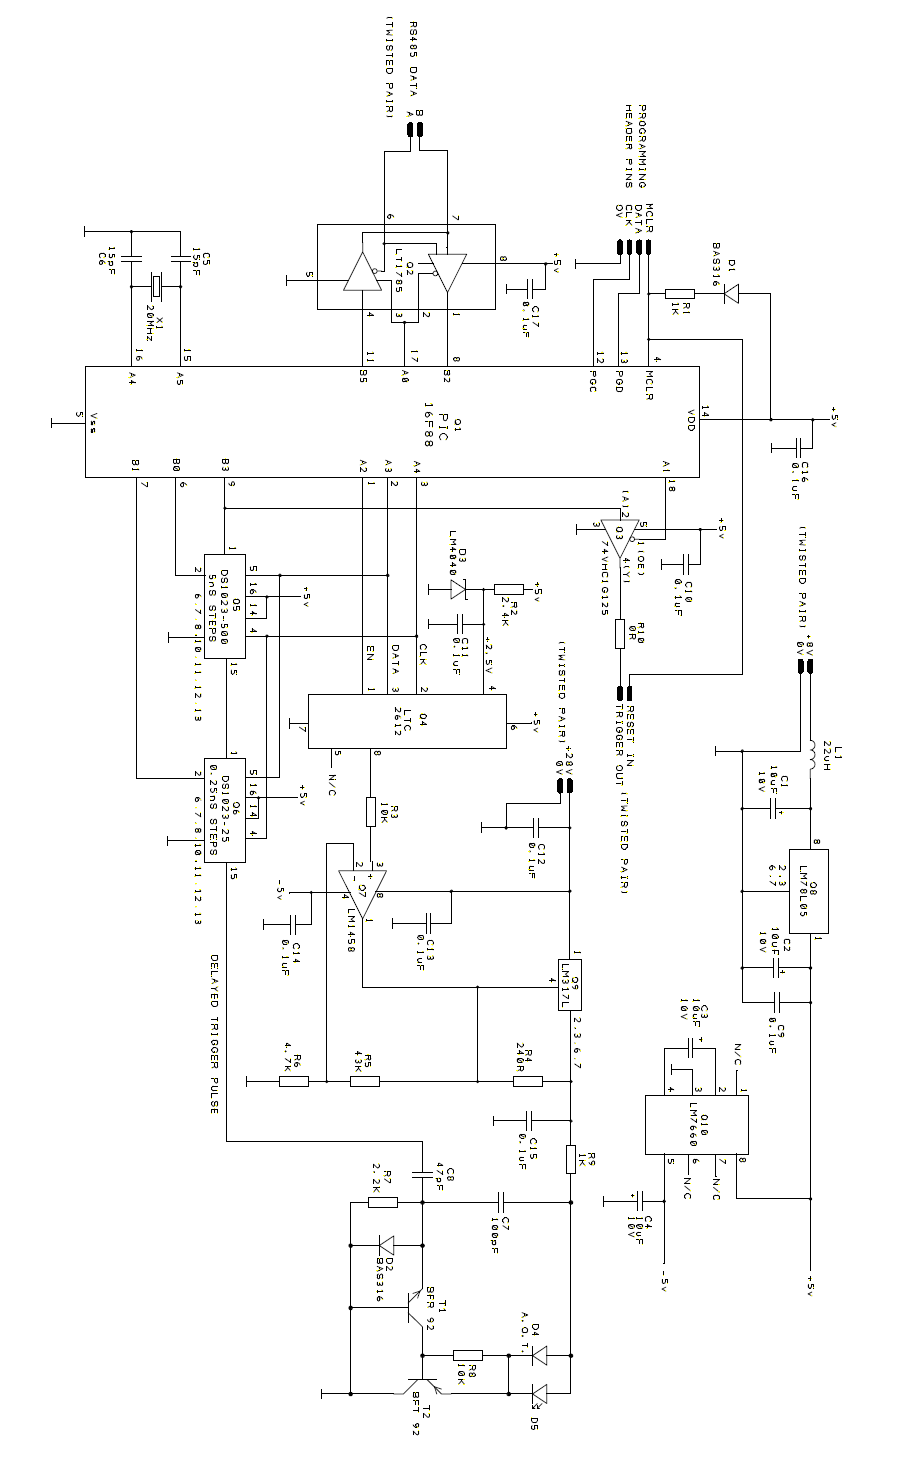
\includegraphics[width=\linewidth]{figures/pulserhead_schematic.png}
\subsection*{Pulserhead schematics}
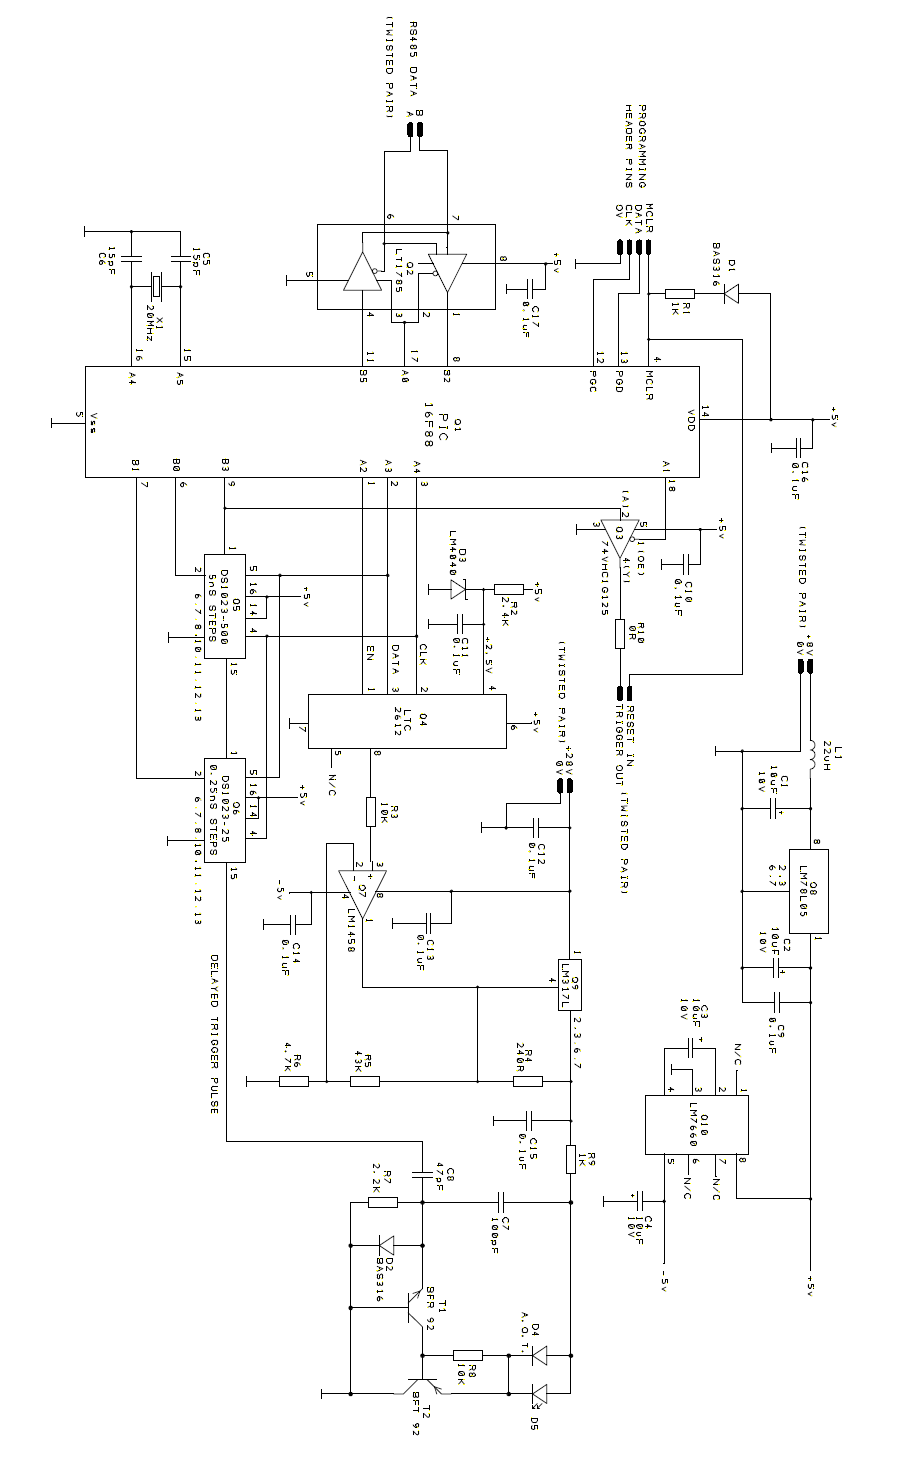
\includegraphics[width=\linewidth]{figures/pulserhead_schematic.png}
%
% Control codes
%
\section{Internal control codes}
\ref{app:internal_codes_design}
The control box will has an integral Raspberry Pi computer running the control program (written in python). The Raspberry Pi is accessible remotely via Ethernet. A USB port for direct control via a laptop is available.

The control codes are given here for reference (although it is recommended to use the python code available):
\begin{itemize}
\item	G= numberlo		
\item H= numberhi
\item I= singleselect
\item L= heighthi
\item M= heightlo
\item P= loadheight
\item a= continuous
\item d= triggerdelay5ns
\item e= triggerdelay025nS
\item g= run
\item x= stop
\item R=reset
\end{itemize}

Slave boards are individually assigned a unique number in the range 1 to 26. For example: to send commands to board 5 send ‘I’ ‘5’, a reply of ‘B5’ will be received. Subsequent commands will go to board 5 until another board is selected. A master hard reset of all slave boards is available via ‘R’, which will reset all the remote slave boards irrespective of the previous board selection.

Number of pulses is set with ‘G’ and ‘H’.

Pulse amplitude is selected with ‘L’ and  ‘M’ and loaded with ‘P’.

A sequence is initiated with ‘g’ or  continuous output with ‘a’.               

Output can be stopped at any time with ‘x’.
%
% Pulser head encapsulation design
%
\section{Pulserhead encapsulation design}
\ref{app:pulserhead_design}
\subsection*{Pulserhead base}
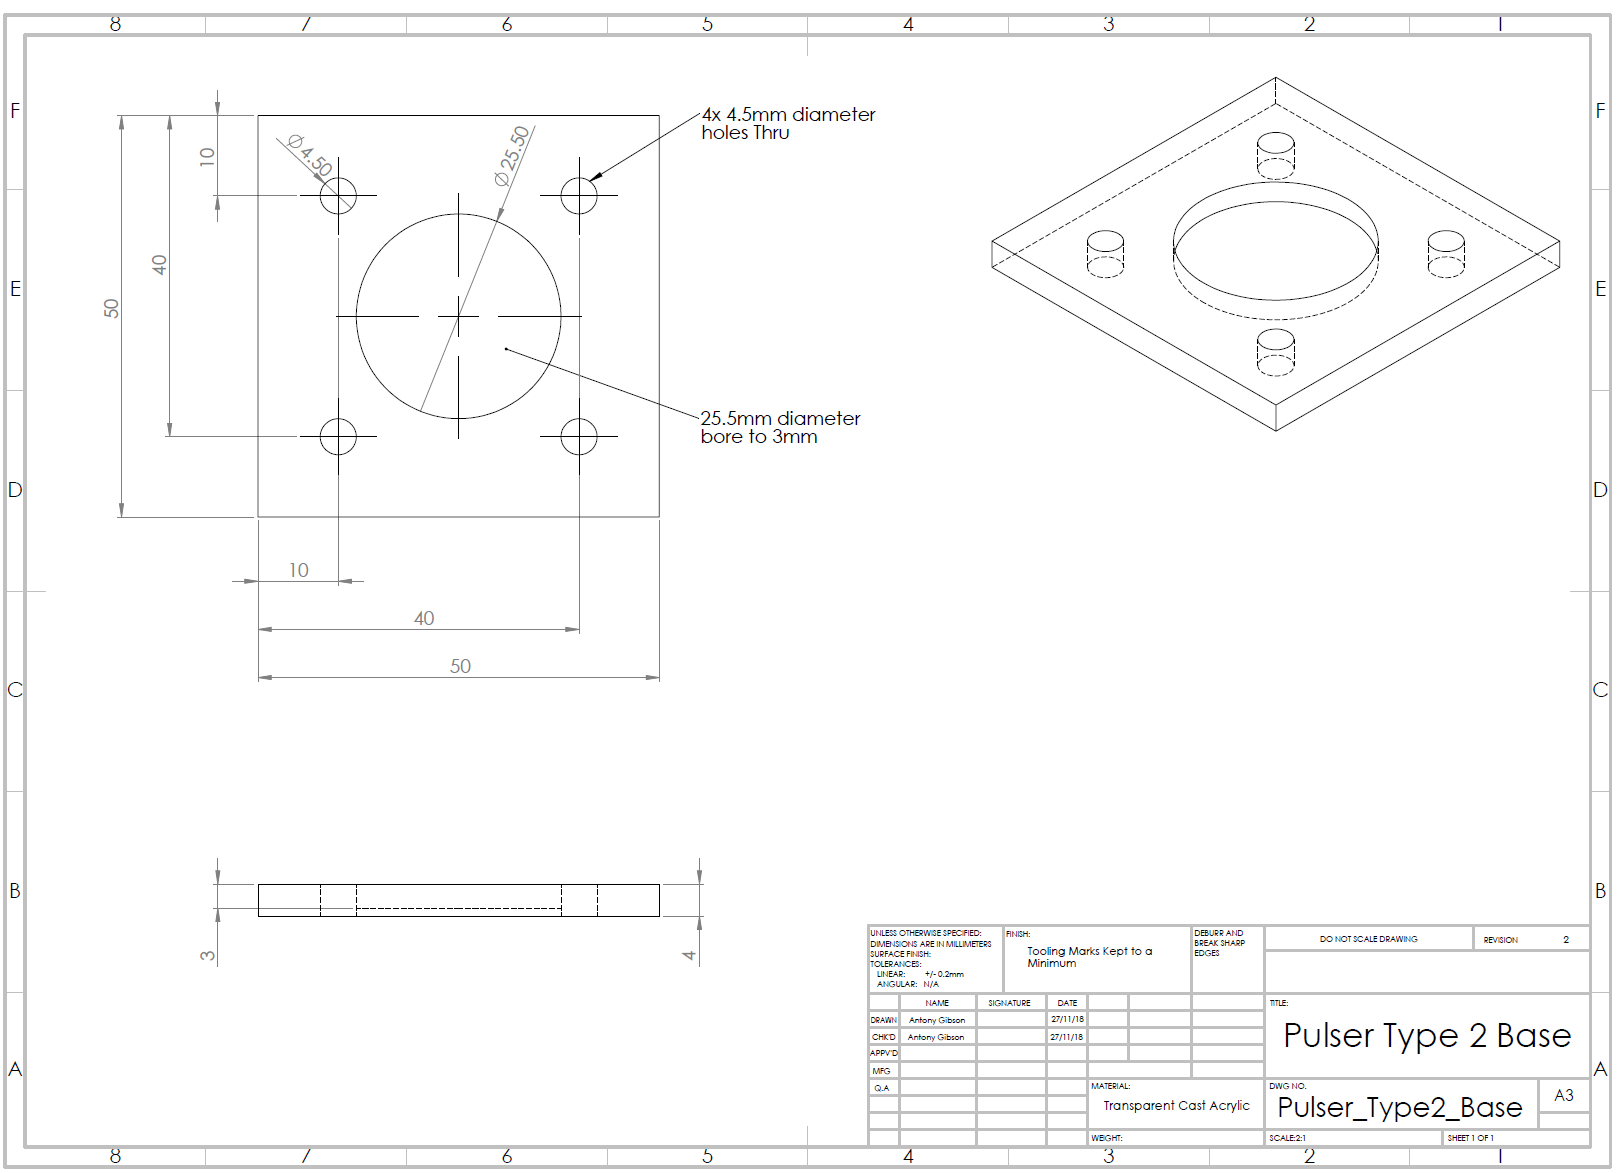
\includegraphics[width=\linewidth]{figures/pulserhead_base.png}
\subsection*{Pulserhead tube}
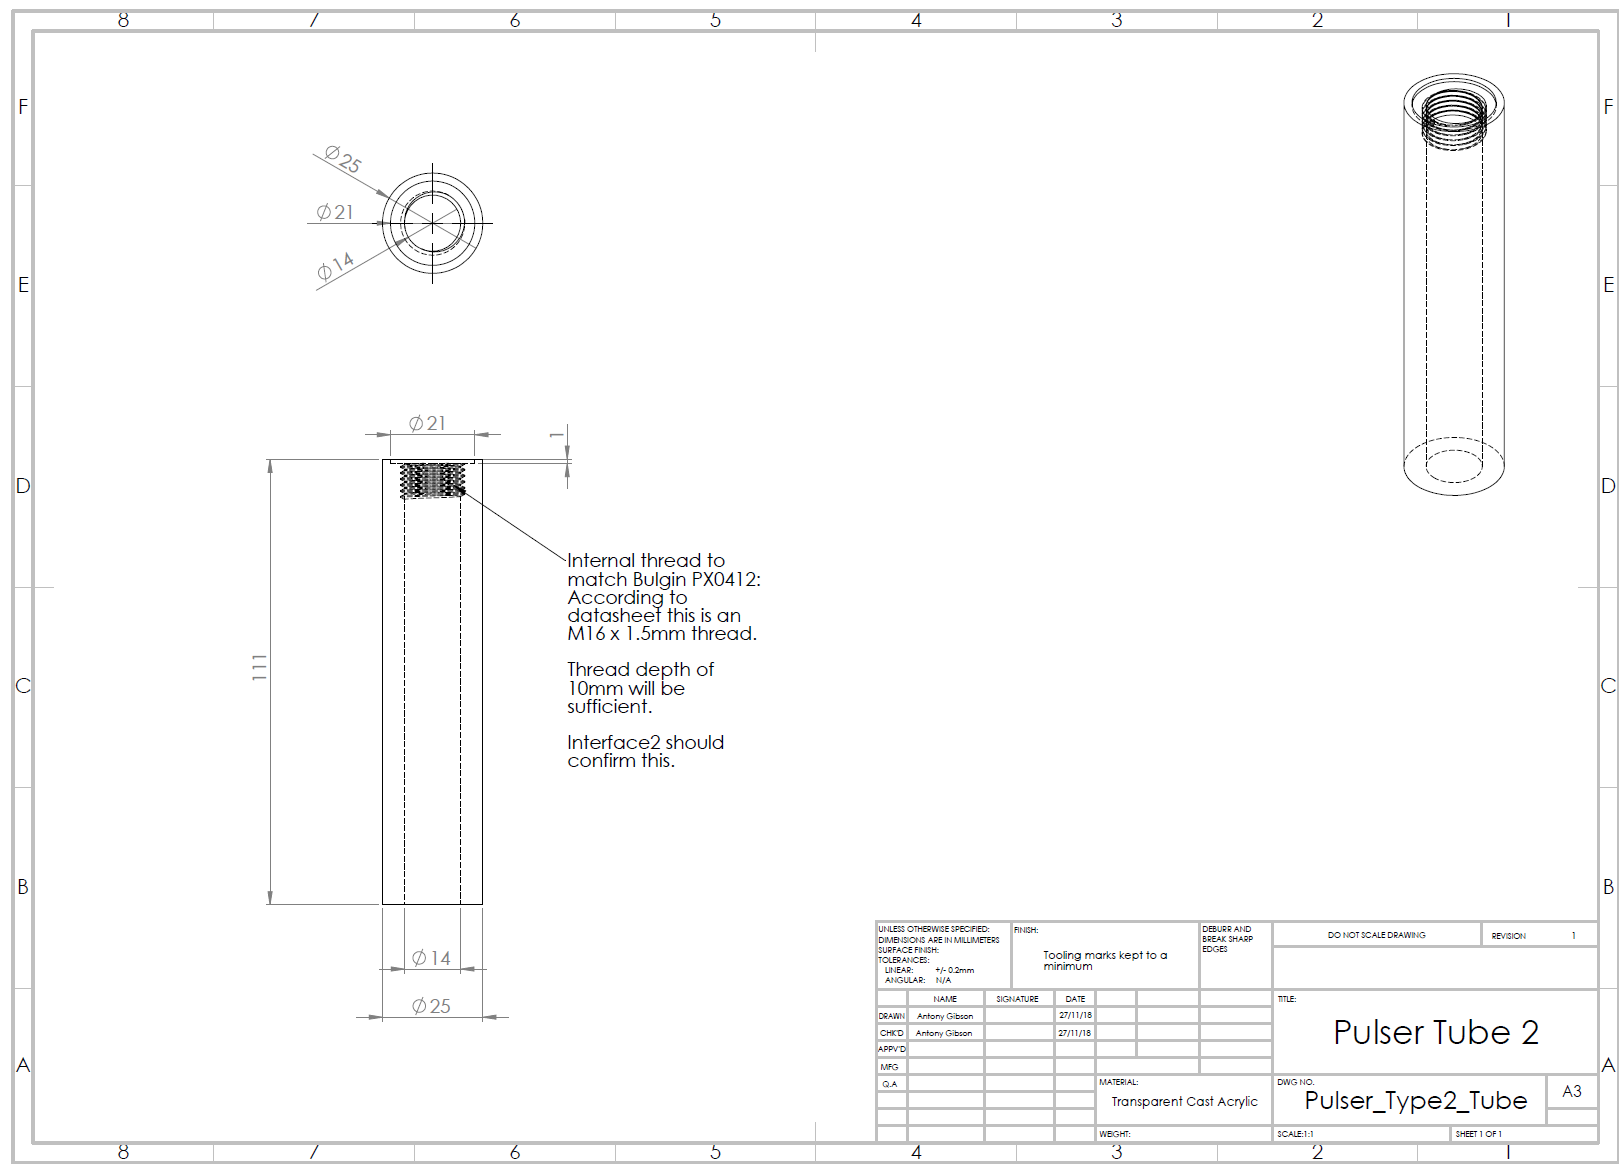
\includegraphics[width=\linewidth]{figures/pulserhead_tube.png}
